\documentclass[12pt]{article}

\usepackage{sbc-template}
\usepackage{graphicx,url}
\usepackage[utf8]{inputenc}
\usepackage[brazil]{babel}
\usepackage{amsmath}
\usepackage{booktabs}
\usepackage{float}

\sloppy

\title{Estudo Comparativo Experimental entre Algoritmo Genético e Simulated Annealing no Problema da Mochila 0/1}

\author{Nicolas S. Pinheiro\inst{1}, Marcos Vinicius M. Costa\inst{1}, Samuel Mota\inst{1}}

\address{
Universidade Federal do Acre -- UFAC\\
Centro de Ciências Exatas e Tecnológicas -- CCET\\
Curso de Sistemas de Informação\\
Rio Branco -- AC -- Brasil\\
\email{\{nicolas.pinheiro, moraes.marcos, samuel.mota\}@sou.ufac.br}
}

\begin{document}

\maketitle

\begin{abstract}
This paper presents an extensive empirical study comparing Genetic Algorithm (GA) and Simulated Annealing (SA) metaheuristics applied to the 0/1 Knapsack Problem. Following a rigorous experimental methodology, we analyze parameter sensitivity across 8 configurations for GA and 5 configurations for SA over 90 benchmark instances generated via the Pisinger algorithm ($n \in \{20, 50, 100\}$, uncorrelated, weakly, and strongly correlated). Exact global optima were computed via Dynamic Programming as reference. After evaluating 11,700 runs, \texttt{GA\_POP\_200} emerged as the best GA variant (mean gap 0.0245\%, optimal rate 67.78\%), while \texttt{SA\_COOL\_SLOW} ($\alpha=0.999$) was the best SA variant (mean gap 0.3889\%, optimal rate 31.11\%, with exactly 10,000 executed iterations). Direct comparison demonstrates that GA achieves superior solution quality through population diversity and crossover recombination, whereas SA provides a significantly lower computational runtime, establishing a clear trade-off between search quality and computational budget.
\end{abstract}

\begin{resumo}
Este artigo apresenta um estudo experimental comparando as metaheurísticas Algoritmo Genético (GA) e Simulated Annealing (SA) aplicadas ao Problema da Mochila 0/1. Seguindo uma metodologia experimental estruturada, analisamos a sensibilidade paramétrica de 8 configurações de GA e 5 de SA em 90 instâncias sintéticas geradas pelo algoritmo de Pisinger ($n \in \{20, 50, 100\}$, não correlacionadas, fracamente e fortemente correlacionadas). As soluções ótimas exatas foram obtidas via Programação Dinâmica como referência. Após 11.700 execuções, a variante \texttt{GA\_POP\_200} consolidou-se como a melhor configuração do GA (gap médio de 0,0245\% e taxa de ótimo de 67,78\%), enquanto a \texttt{SA\_COOL\_SLOW} ($\alpha=0.999$) foi a melhor do SA (gap médio de 0,3889\%, taxa de ótimo de 31,11\% e 10.000 iterações efetivamente executadas). A comparação direta evidencia que o GA atinge qualidade superior devido à diversidade populacional e recombinação por crossover, enquanto o SA oferece menor tempo de execução, estabelecendo um nítido \textit{trade-off} entre qualidade de busca e orçamento computacional.
\end{resumo}

\section{Introdução}

Problemas de otimização combinatória desempenham um papel central na Ciência da Computação, Engenharia e Pesquisa Operacional. Em geral, consistem em selecionar uma solução viável de qualidade máxima dentro de um conjunto discreto de alternativas que cresce exponencialmente com a dimensão do problema. Quando os algoritmos exatos se tornam computacionalmente inviáveis em instâncias de grande porte, metaheurísticas surgem como alternativas eficientes para obter soluções aproximadas de alta qualidade em tempo razoável \cite{talbi2009}.

Dentre os problemas clássicos de otimização combinatória, destaca-se o Problema da Mochila 0/1 (\textit{0/1 Knapsack Problem}). O objetivo consiste em selecionar um subconjunto de itens, cada qual dotado de peso e valor, de forma a maximizar a soma dos valores sem que a soma dos pesos ultrapasse a capacidade máxima da mochila \cite{ortools_knapsack}.

Este trabalho conduz uma investigação experimental sistemática comparando duas metaheurísticas de paradigmas distintos: o Algoritmo Genético (GA), baseado em população, e o Simulated Annealing (SA), baseado em solução única com aceitação estocástica. O estudo divide-se em quatro partes fundamentais:
\begin{enumerate}
    \item Avaliação de sensibilidade paramétrica do Algoritmo Genético e seleção da melhor configuração (\texttt{best\_GA});
    \item Avaliação de sensibilidade paramétrica do Simulated Annealing e seleção da melhor configuração (\texttt{best\_SA});
    \item Comparação direta e detalhada dos \textit{trade-offs} entre \texttt{best\_GA} e \texttt{best\_SA};
    \item Documentação completa e discussão fundamentada dos mecanismos de busca no presente artigo no padrão SBC.
\end{enumerate}

\section{Fundamentação Teórica}

\subsection{Problema da Mochila 0/1}

Formalmente, dada uma instância com $n$ itens, onde cada item $i$ possui valor $v_i > 0$ e peso $w_i > 0$, e uma mochila de capacidade $C > 0$, o Problema da Mochila 0/1 é formulado como:

\begin{equation}
\max \sum_{i=1}^{n} v_i x_i
\end{equation}
sujeito a:
\begin{equation}
\sum_{i=1}^{n} w_i x_i \leq C, \quad \text{com } x_i \in \{0,1\}, \; \forall i \in \{1, \ldots, n\}.
\end{equation}

Uma solução é representada por um vetor binário $x = (x_1, x_2, \dots, x_n)$, onde $x_i = 1$ indica a inclusão do item $i$ e $x_i = 0$ sua exclusão.

\subsection{Algoritmo Genético (GA)}

O Algoritmo Genético é uma metaheurística evolutiva inspirada na seleção natural e genética das espécies \cite{talbi2009}. Opera sobre uma população de indivíduos (vetores binários). A cada geração, indivíduos são selecionados com base no seu valor de aptidão (\textit{fitness}), sofrem recombinação (crossover) com probabilidade $P_c$, mutação por inversão de bit com probabilidade $P_m$, e o melhor indivíduo é preservado para a geração seguinte via elitismo.

\subsection{Simulated Annealing (SA)}

O Simulated Annealing é uma metaheurística de solução única inspirada no processo físico de recozimento de metais \cite{talbi2009}. A partir de uma solução inicial $x$, a cada iteração uma solução vizinha $x'$ é gerada por alteração pontual (flip de 1 bit). Se a solução vizinha melhora o valor total ($\Delta = V(x') - V(x) \geq 0$), ela é aceita incondicionalmente. Se resulta em piora ($\Delta < 0$), ela é aceita probabilisticamente de acordo com o critério de Metropolis:
\begin{equation}
P(\text{aceitar}) = \exp\left(\frac{\Delta}{T}\right)
\end{equation}
onde $T$ representa a temperatura atual, que decai a cada iteração seguindo uma taxa de resfriamento geométrico $T_{k+1} = \alpha T_k$.

\section{Metodologia Experimental}

\subsection{Instâncias e Valor Ótimo de Referência}

Para garantir rigor e reprodutibilidade, utilizamos o gerador baseado no algoritmo de Pisinger \cite{pisinger2005, pisinger_generator}. Foram geradas 90 instâncias divididas em:
\begin{itemize}
    \item \textbf{Tamanhos ($n$):} 20, 50 e 100 itens;
    \item \textbf{Classes de correlação:} Não correlacionadas (\textit{uncorrelated}), Fracamente correlacionadas (\textit{weakly correlated}) e Fortemente correlacionadas (\textit{strongly correlated});
    \item \textbf{Quantidade:} 10 instâncias por grupo (3 tamanhos $\times$ 3 correlações $\times$ 10 instâncias).
\end{itemize}
O valor ótimo de cada instância ($V_{\text{ótimo}}$) foi previamente computado de forma exata via Programação Dinâmica com complexidade $O(nC)$, servindo exclusivamente como referência offline para cálculo de métricas de desempenho.

\subsection{Ambiente Experimental e Estratégia de Reparo}

Para evitar viés experimental, ambas as metaheurísticas compartilham rigorosamente a mesma estratégia de representação e reparo de soluções inviáveis: caso $\sum w_i x_i > C$, os itens presentes na solução de menor razão valor/peso ($v_i / w_i$) são sequencialmente removidos até que a restrição de capacidade seja atendida.

Cada configuração algorítmica foi executada 10 vezes por instância utilizando sementes pseudorrandômicas determinísticas ($seed = BASE\_SEED + inst\_idx \times 1000 + run\_idx$). O vizinho no SA é gerado por flip de 1 bit e, se inviável, submetido ao reparo por razão valor/peso.

\subsection{Métricas de Avaliação e Critério de Seleção}

As métricas registradas nas 11.700 execuções foram agregadas em dois níveis estatísticos (calculando-se primeiramente a média das 10 repetições de cada uma das 90 instâncias e, subsequentemente, os desvios e médias globais sobre as 90 instâncias):
\begin{itemize}
    \item \textbf{Gap percentual (\%):} $\frac{V_{\text{ótimo}} - V_{\text{encontrado}}}{V_{\text{ótimo}}} \times 100$;
    \item \textbf{Taxa de ótimo (\%):} Proporção de execuções que atingiram $V_{\text{encontrado}} = V_{\text{ótimo}}$ (gap $= 0\%$);
    \item \textbf{Tempo de execução (ms):} Tempo computacional despendido em milissegundos;
    \item \textbf{Número de avaliações da função objetivo:} Total de soluções avaliadas durante a busca;
    \item \textbf{Iterações efetivamente executadas:} Gerações no GA ou iterações realizadas até o congelamento no SA.
\end{itemize}

\paragraph{Critério Formal para Seleção das Melhores Configurações (\texttt{best\_GA} e \texttt{best\_SA}):}
A definição da melhor configuração para cada algoritmo obedeceu rigorosamente à seguinte hierarquia:
\begin{enumerate}
    \item \textbf{Critério Primário:} Menor gap médio em relação ao ótimo ($G_{\text{médio}}$);
    \item \textbf{Critério de Desempate:} Maior taxa de obtenção do ótimo global ($T_{\text{ótimo}}$);
    \item \textbf{Análise de Eficiência:} Menor custo em tempo ($t_{\text{ms}}$) e avaliações ($N_{\text{aval}}$) avaliados posteriormente na fronteira de Pareto, sem comprometer os critérios primários de qualidade.
\end{enumerate}

\subsection{Configurações do Algoritmo Genético (GA)}

Foram avaliadas 8 variações controladas do GA (alterando um único parâmetro por variante em relação à base \texttt{GA\_BASE}):
\begin{enumerate}
    \item \texttt{GA\_BASE}: População $N=100$, 100 gerações (20.200 avaliações), $P_c=0.80$, $P_m=1/n$, torneio $k=3$, elitismo habilitado;
    \item \texttt{GA\_POP\_50}: População reduzida $N=50$ (10.100 avaliações);
    \item \texttt{GA\_POP\_200}: População ampliada $N=200$ (40.400 avaliações);
    \item \texttt{GA\_CROSS\_060}: Taxa de crossover reduzida $P_c=0.60$;
    \item \texttt{GA\_CROSS\_095}: Taxa de crossover elevada $P_c=0.95$;
    \item \texttt{GA\_MUT\_LOW}: Taxa de mutação reduzida $P_m=0,5/n$;
    \item \texttt{GA\_MUT\_HIGH}: Taxa de mutação elevada $P_m=2/n$;
    \item \texttt{GA\_TOUR\_5}: Pressão seletiva elevada com torneio $k=5$.
\end{enumerate}

\subsection{Configurações do Simulated Annealing (SA)}

Foram avaliadas 5 variações controladas do SA:
\begin{enumerate}
    \item \texttt{SA\_BASE}: Limite de 10.000 iterações, $T_0=1000.0$, $T_{\min}=0.001$, $\alpha=0.995$;
    \item \texttt{SA\_COOL\_FAST}: Resfriamento rápido $\alpha=0.98$;
    \item \texttt{SA\_COOL\_SLOW}: Resfriamento lento $\alpha=0.999$;
    \item \texttt{SA\_T0\_LOW}: Temperatura inicial menor $T_0=100.0$;
    \item \texttt{SA\_T0\_HIGH}: Temperatura inicial maior $T_0=5000.0$.
\end{enumerate}

\section{Resultados e Discussão}

\subsection{Parte 1 — Sensibilidade dos Parâmetros do Algoritmo Genético}

A Tabela~\ref{tab:ga_summary} resume os resultados médios globais obtidos pelas 8 variações do Algoritmo Genético em todas as 90 instâncias (900 execuções por configuração).

\begin{table}[H]
\centering
\caption{Desempenho comparativo global das configurações do Algoritmo Genético.}
\label{tab:ga_summary}
\resizebox{\textwidth}{!}{%
\begin{tabular}{@{}lrrrr@{}}
\toprule
Configuração GA & \shortstack{Gap Médio\\(\%)} & \shortstack{Taxa de Ótimo\\(\%)} & \shortstack{Tempo Médio\\(ms)} & Avaliações \\
\midrule
\texttt{GA\_POP\_200}  & \textbf{0,0245} & \textbf{67,78\%} & 201,16 & 40.400 \\
\texttt{GA\_MUT\_HIGH} & 0,0252 & 58,56\% & 104,72 & 20.200 \\
\texttt{GA\_CROSS\_095}& 0,0399 & 58,78\% & 103,15 & 20.200 \\
\texttt{GA\_BASE}      & 0,0423 & 55,67\% & 100,78 & 20.200 \\
\texttt{GA\_CROSS\_060}& 0,0560 & 51,00\% & 97,76  & 20.200 \\
\texttt{GA\_MUT\_LOW}  & 0,0749 & 45,00\% & 95,76  & 20.200 \\
\texttt{GA\_TOUR\_5}   & 0,0805 & 46,00\% & 105,14 & 20.200 \\
\texttt{GA\_POP\_50}   & 0,1093 & 41,78\% & 50,12  & 10.100 \\
\bottomrule
\end{tabular}
}%
\end{table}

\begin{figure}[H]
\centering
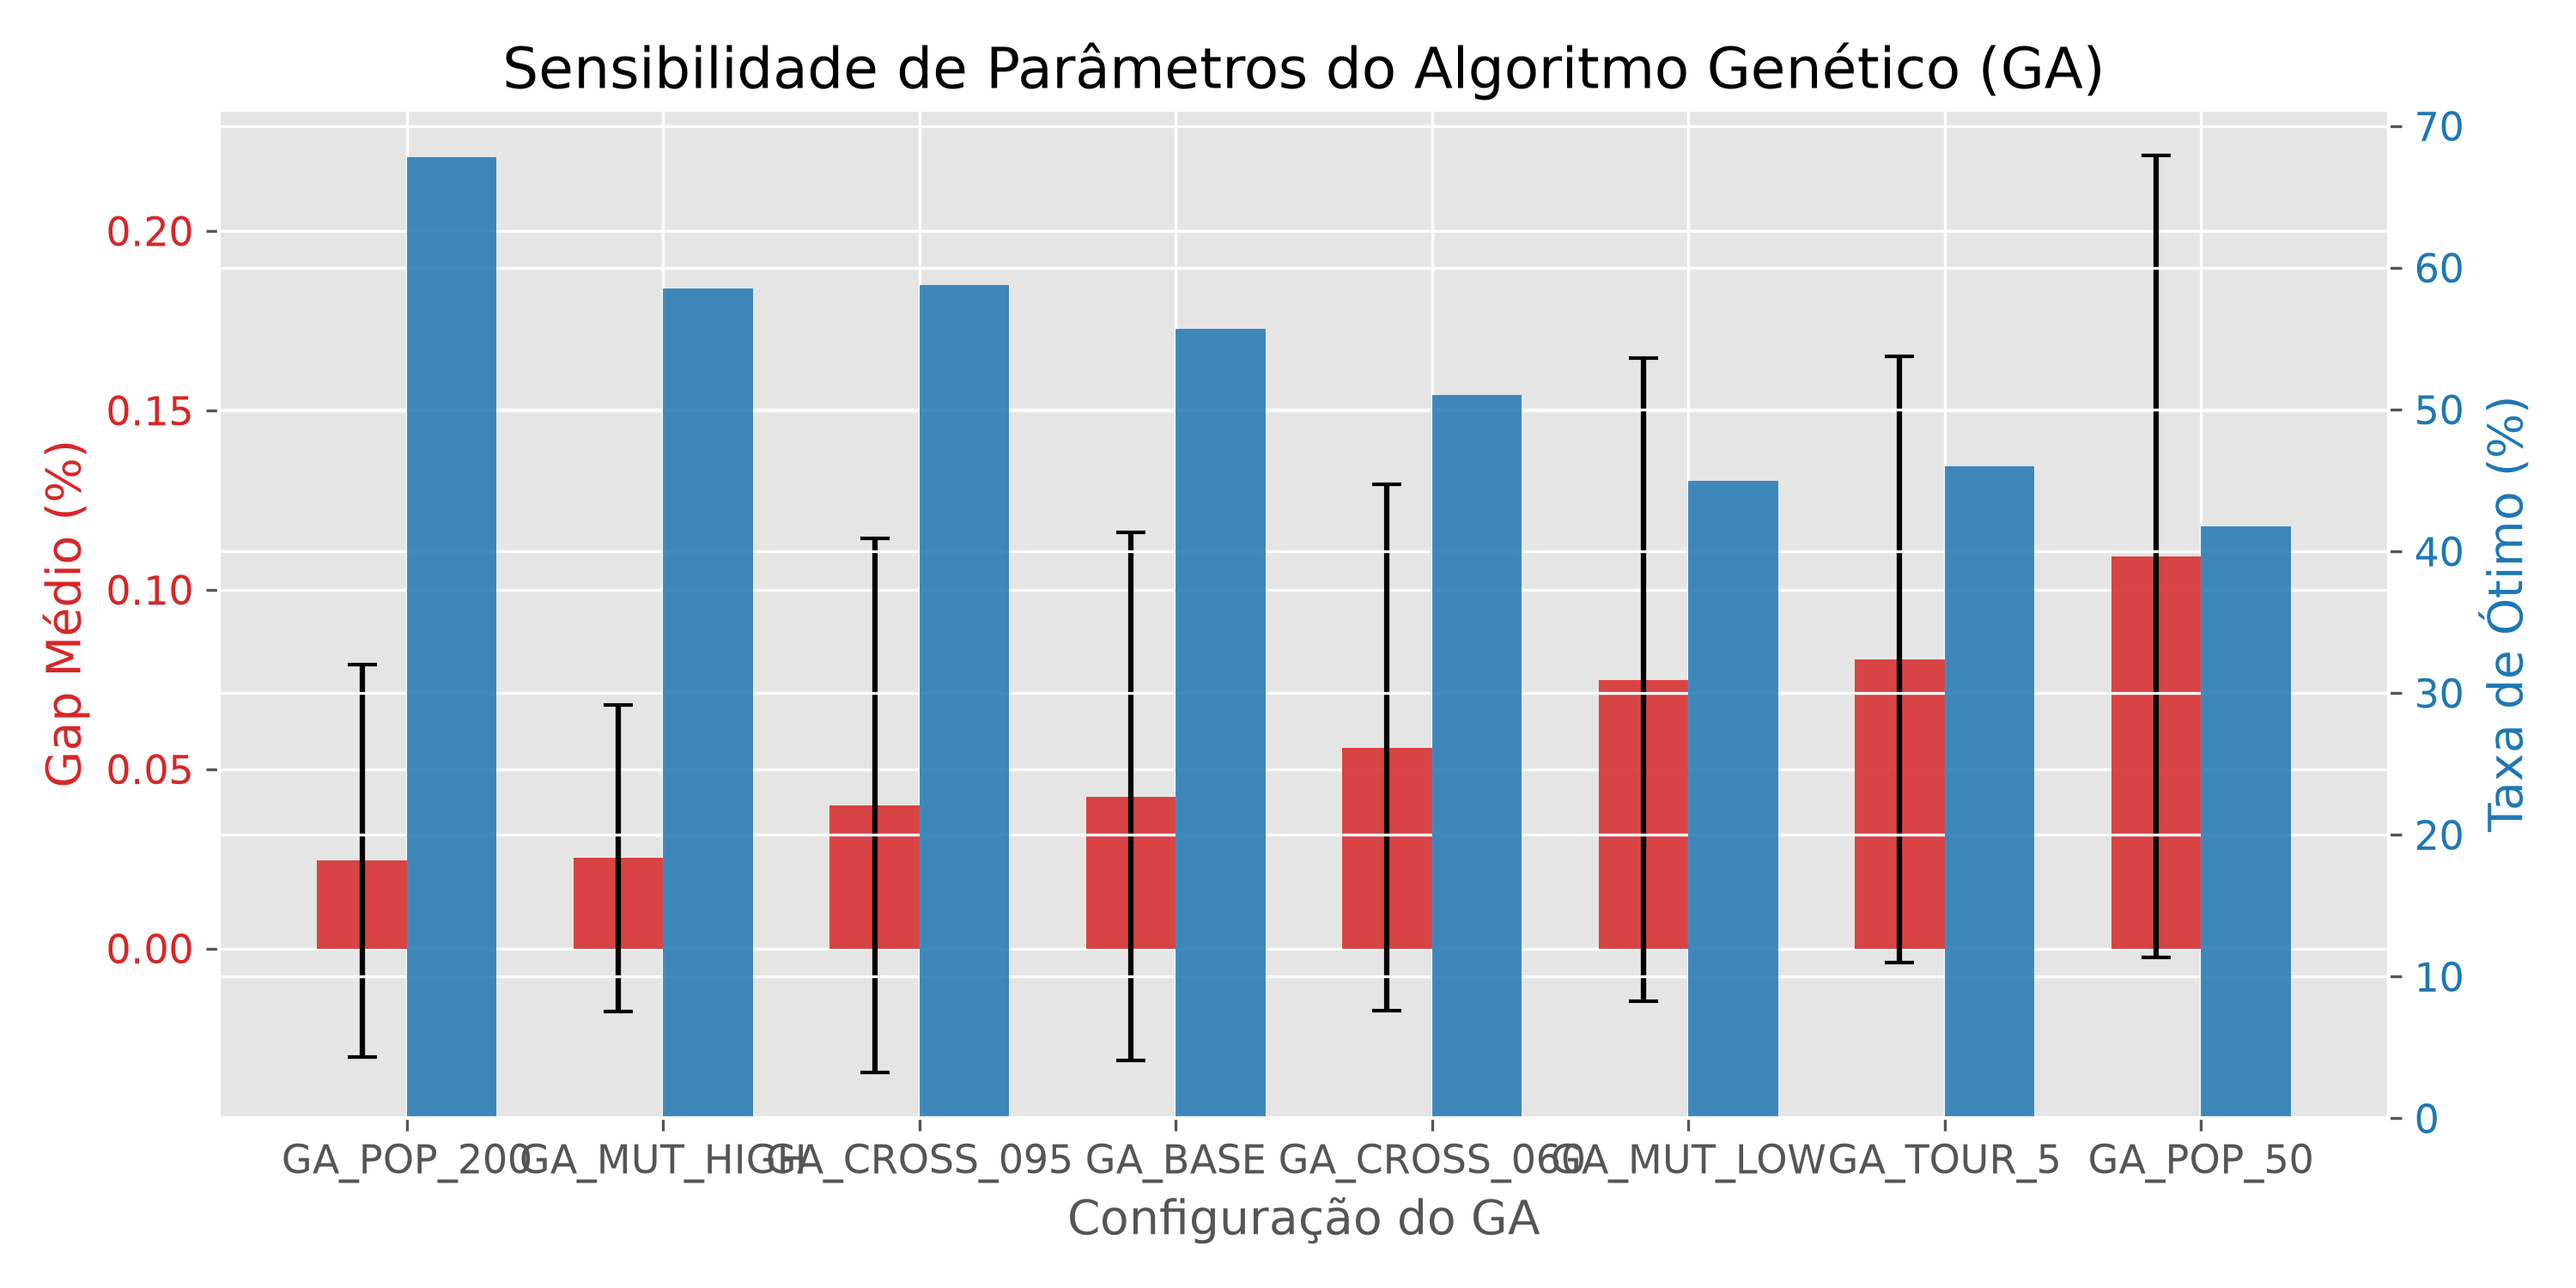
\includegraphics[width=0.85\textwidth]{../results/figures/ga_config_comparison.png}
\caption{Sensibilidade de Parâmetros do Algoritmo Genético (Gap Médio com desvio padrão e Taxa de Ótimo).}
\label{fig:ga_config}
\end{figure}

\paragraph{Análise dos Mecanismos do GA:}
\begin{itemize}
    \item \textbf{Tamanho Populacional ($N=200$ vs $N=50$):} O aumento populacional para 200 indivíduos expandiu a amostragem inicial do espaço de busca. O comportamento observado é compatível com a hipótese de que uma população maior preserva a diversidade por mais gerações, permitindo ao crossover combinar esquemas heterogêneos. O gap médio diminuiu de 0,1093\% ($N=50$) para 0,0245\% ($N=200$) e a taxa de ótimo elevou-se de 41,78\% para 67,78\%, acompanhada do aumento nas avaliações (40.400 vs 10.100).
    \item \textbf{Taxa de Mutação ($2/n$ vs $0,5/n$):} A variante com maior mutação (\texttt{GA\_MUT\_HIGH}) atingiu gap médio de 0,0252\%, próximo ao \texttt{GA\_POP\_200}, consumindo metade do orçamento de avaliações (20.200). Esse resultado sugere que a diversificação induzida por mutação frequente atuou na prevenção de estagnações locais.
    \item \textbf{Pressão Seletiva ($k=5$ vs $k=3$):} A elevação do tamanho do torneio para $k=5$ associou-se a um aumento do gap para 0,0805\%, comportamento condizente com os efeitos teóricos da convergência prematura sob alta pressão seletiva.
\end{itemize}

Com base nesses resultados experimentais, a configuração \textbf{\texttt{GA\_POP\_200}} foi selecionada como a melhor variante em qualidade pura (\texttt{best\_GA}).

\subsection{Parte 2 — Sensibilidade dos Parâmetros do Simulated Annealing}

A Tabela~\ref{tab:sa_summary} apresenta os resultados globais obtidos pelas 5 variações do Simulated Annealing.

\begin{table}[H]
\centering
\caption{Desempenho comparativo global das configurações do Simulated Annealing.}
\label{tab:sa_summary}
\resizebox{\textwidth}{!}{%
\begin{tabular}{@{}lrrrrr@{}}
\toprule
Configuração SA & \shortstack{Gap Médio\\(\%)} & \shortstack{Taxa de Ótimo\\(\%)} & \shortstack{Tempo Médio\\(ms)} & \shortstack{Iterações\\Efetivas} & Avaliações \\
\midrule
\texttt{SA\_COOL\_SLOW} & \textbf{0,3889} & \textbf{31,11\%} & 60,46 & 10.000 & 20.002 \\
\texttt{SA\_T0\_HIGH}   & 0,8521 & 21,67\% & 18,38 & 3.078  & 6.158 \\
\texttt{SA\_BASE}      & 0,8810 & 20,44\% & 16,57 & 2.757  & 5.516 \\
\texttt{SA\_COOL\_FAST} & 1,7841 & 12,11\% & 4,10  & 684    & 1.370 \\
\texttt{SA\_T0\_LOW}    & 2,0846 & 13,22\% & 14,08 & 2.297  & 4.596 \\
\bottomrule
\end{tabular}
}%
\end{table}

\begin{figure}[H]
\centering
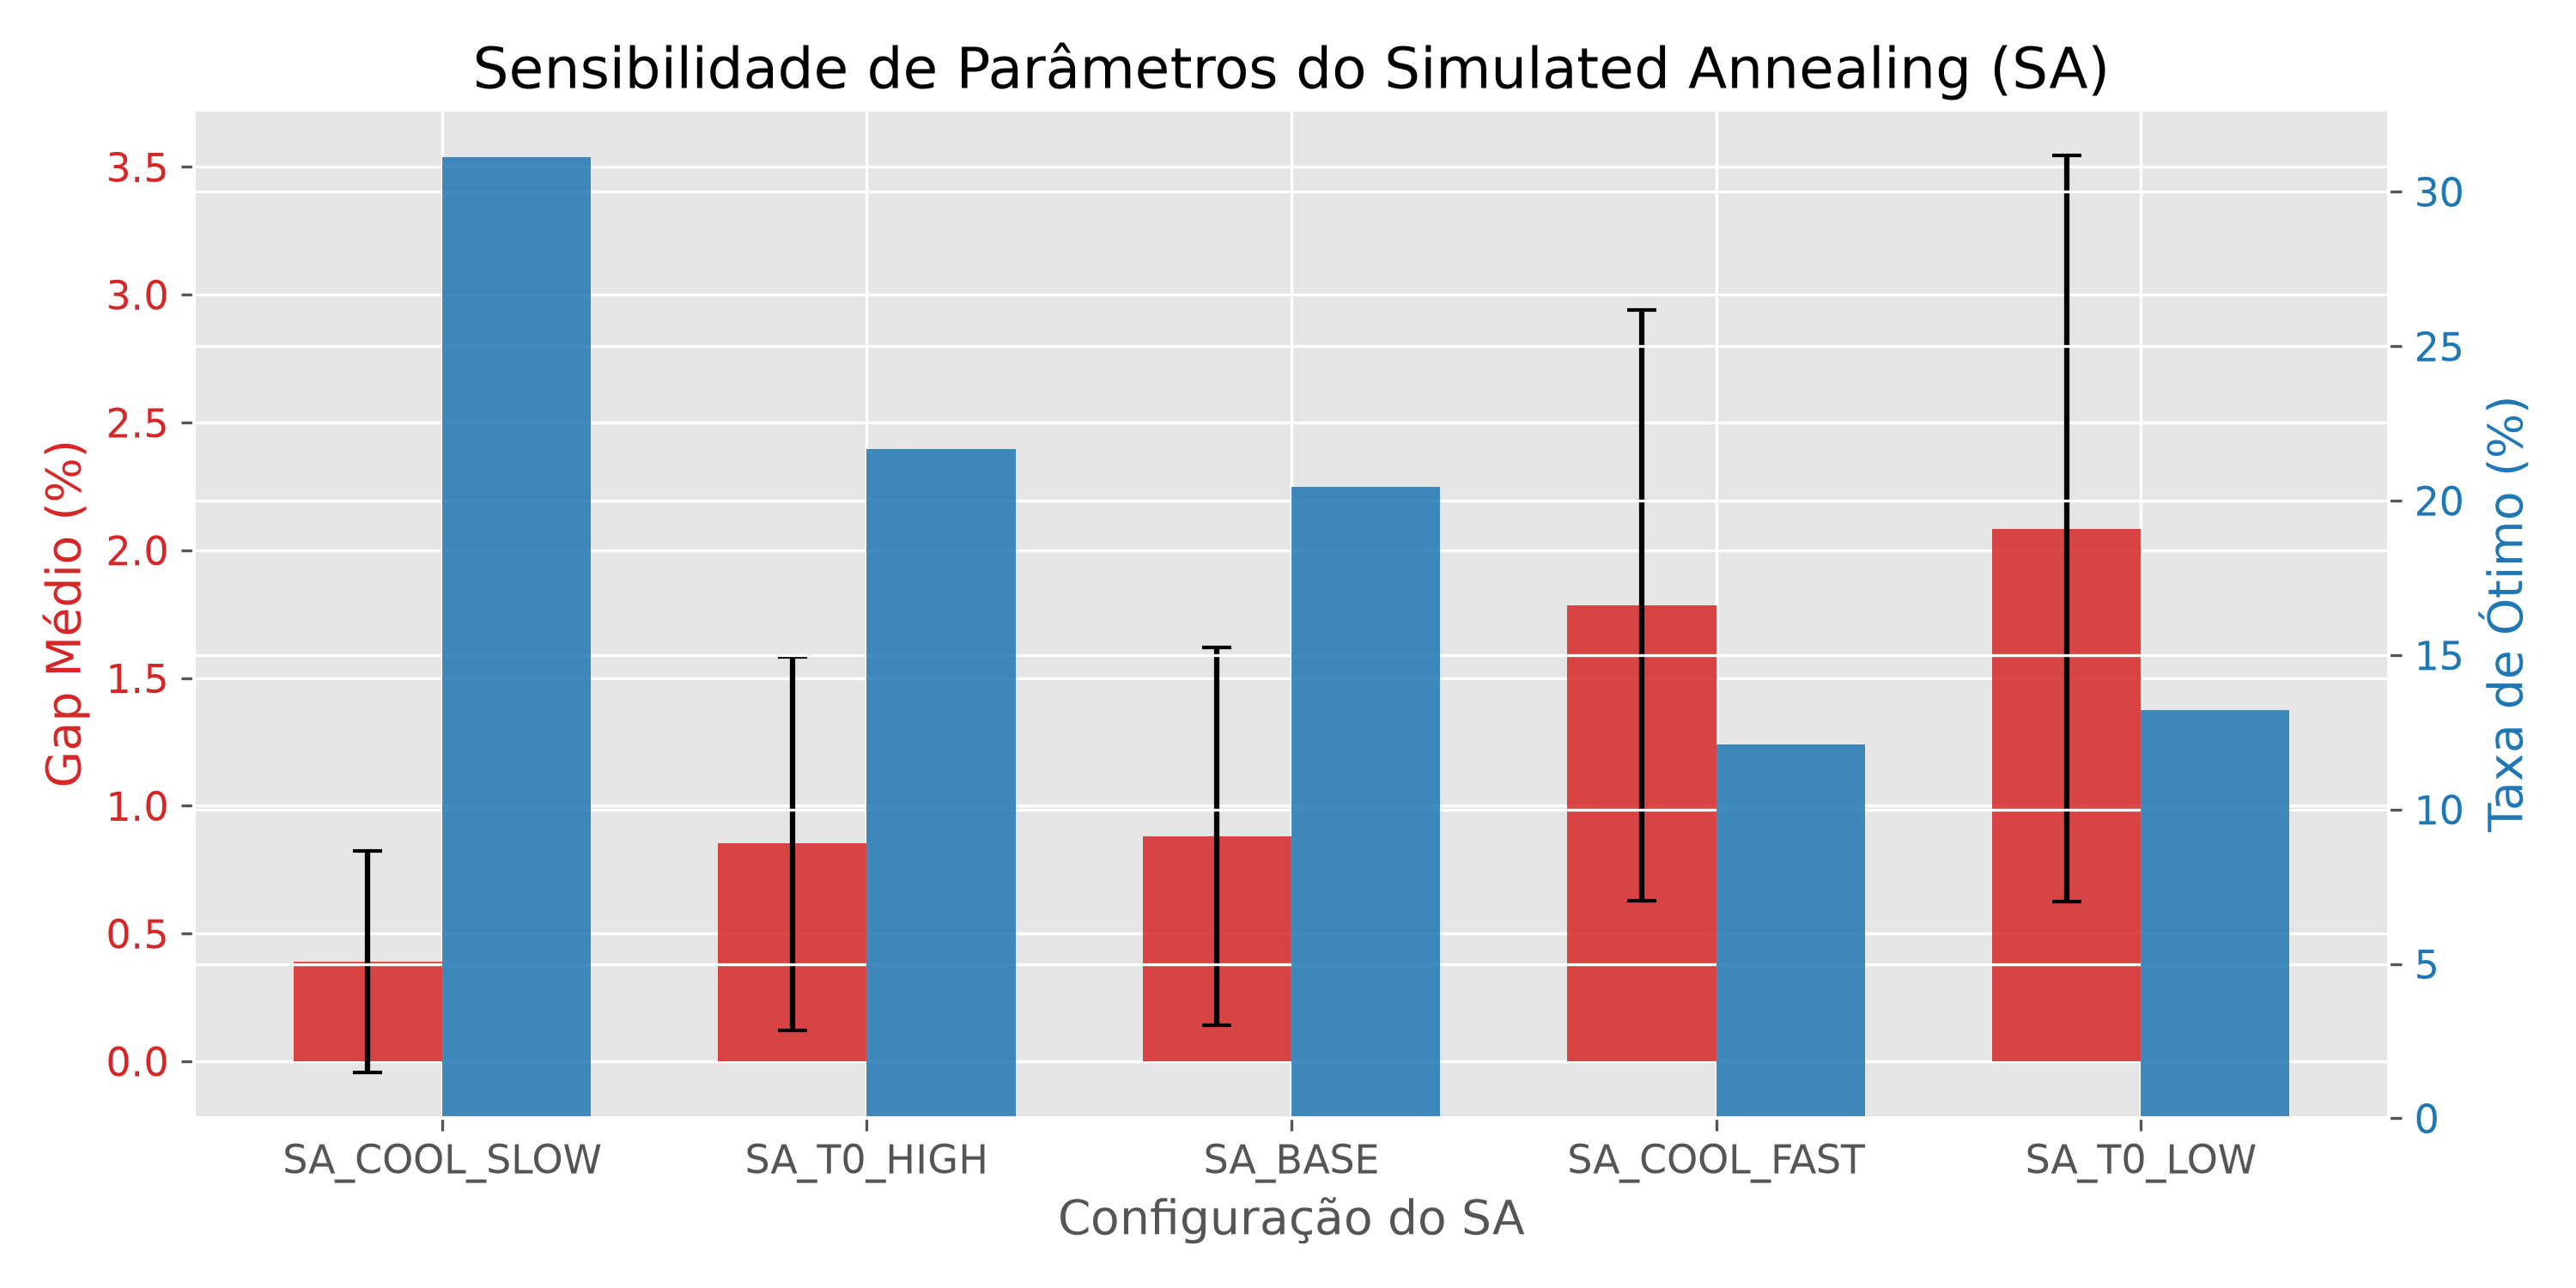
\includegraphics[width=0.85\textwidth]{../results/figures/sa_config_comparison.png}
\caption{Sensibilidade de Parâmetros do Simulated Annealing (Gap Médio com desvio padrão e Taxa de Ótimo).}
\label{fig:sa_config}
\end{figure}

\paragraph{Análise dos Mecanismos do SA:}
\begin{itemize}
    \item \textbf{Taxa de Resfriamento e Iterações Reais:} A instrumentação exata revelou que a variação de $\alpha$ altera dramaticamente o total de iterações antes do congelamento ($T < 0.001$). Na configuração \texttt{SA\_COOL\_FAST} ($\alpha=0.98$), o congelamento ocorreu com apenas 684 iterações reais (1.370 avaliações), degradando o gap para 1,7841\%. Já a variante \texttt{SA\_COOL\_SLOW} ($\alpha=0.999$) estendeu o congelamento até o limite máximo de 10.000 iterações (20.002 avaliações), resultando no menor gap (0,3889\%).
    \item \textbf{Temperatura Inicial ($T_0=100$ vs $T_0=5000$):} Temperaturas iniciais mais baixas (\texttt{SA\_T0\_LOW}) tornaram o algoritmo excessivamente guloso no início, congelando em 2.297 iterações e elevando o gap para 2,0846\%.
\end{itemize}

Dessa forma, a variante \textbf{\texttt{SA\_COOL\_SLOW}} foi selecionada como a melhor configuração do SA (\texttt{best\_SA}).

\subsection{Parte 3 — Comparação Final: Melhor GA (\texttt{GA\_POP\_200}) $\times$ Melhor SA (\texttt{SA\_COOL\_SLOW})}

A Tabela~\ref{tab:final_comparison} detalha o confronto final entre \texttt{best\_GA} e \texttt{best\_SA} desagregado pelas dimensões do problema ($n$).

\begin{table}[H]
\centering
\caption{Comparação final entre a melhor configuração de GA e a melhor de SA por tamanho de problema ($n$).}
\label{tab:final_comparison}
\resizebox{\textwidth}{!}{%
\begin{tabular}{@{}crrrrr@{}}
\toprule
$n$ & Algoritmo & \shortstack{Gap Médio\\(\%)} & \shortstack{Taxa de Ótimo\\(\%)} & \shortstack{Tempo Médio\\(ms)} & Avaliações \\
\midrule
20  & \texttt{GA\_POP\_200}  & \textbf{0,0366} & \textbf{78,00\%} & 98,40  & 40.400 \\
20  & \texttt{SA\_COOL\_SLOW}& 0,1476          & 59,00\%          & 27,24  & 20.002 \\
\midrule
50  & \texttt{GA\_POP\_200}  & \textbf{0,0209} & \textbf{70,33\%} & 183,16 & 40.400 \\
50  & \texttt{SA\_COOL\_SLOW}& 0,3675          & 20,67\%          & 53,88  & 20.002 \\
\midrule
100 & \texttt{GA\_POP\_200}  & \textbf{0,0161} & \textbf{55,00\%} & 321,92 & 40.400 \\
100 & \texttt{SA\_COOL\_SLOW}& 0,6517          & 13,67\%          & 100,27 & 20.002 \\
\bottomrule
\end{tabular}
}%
\end{table}

\begin{figure}[H]
\centering
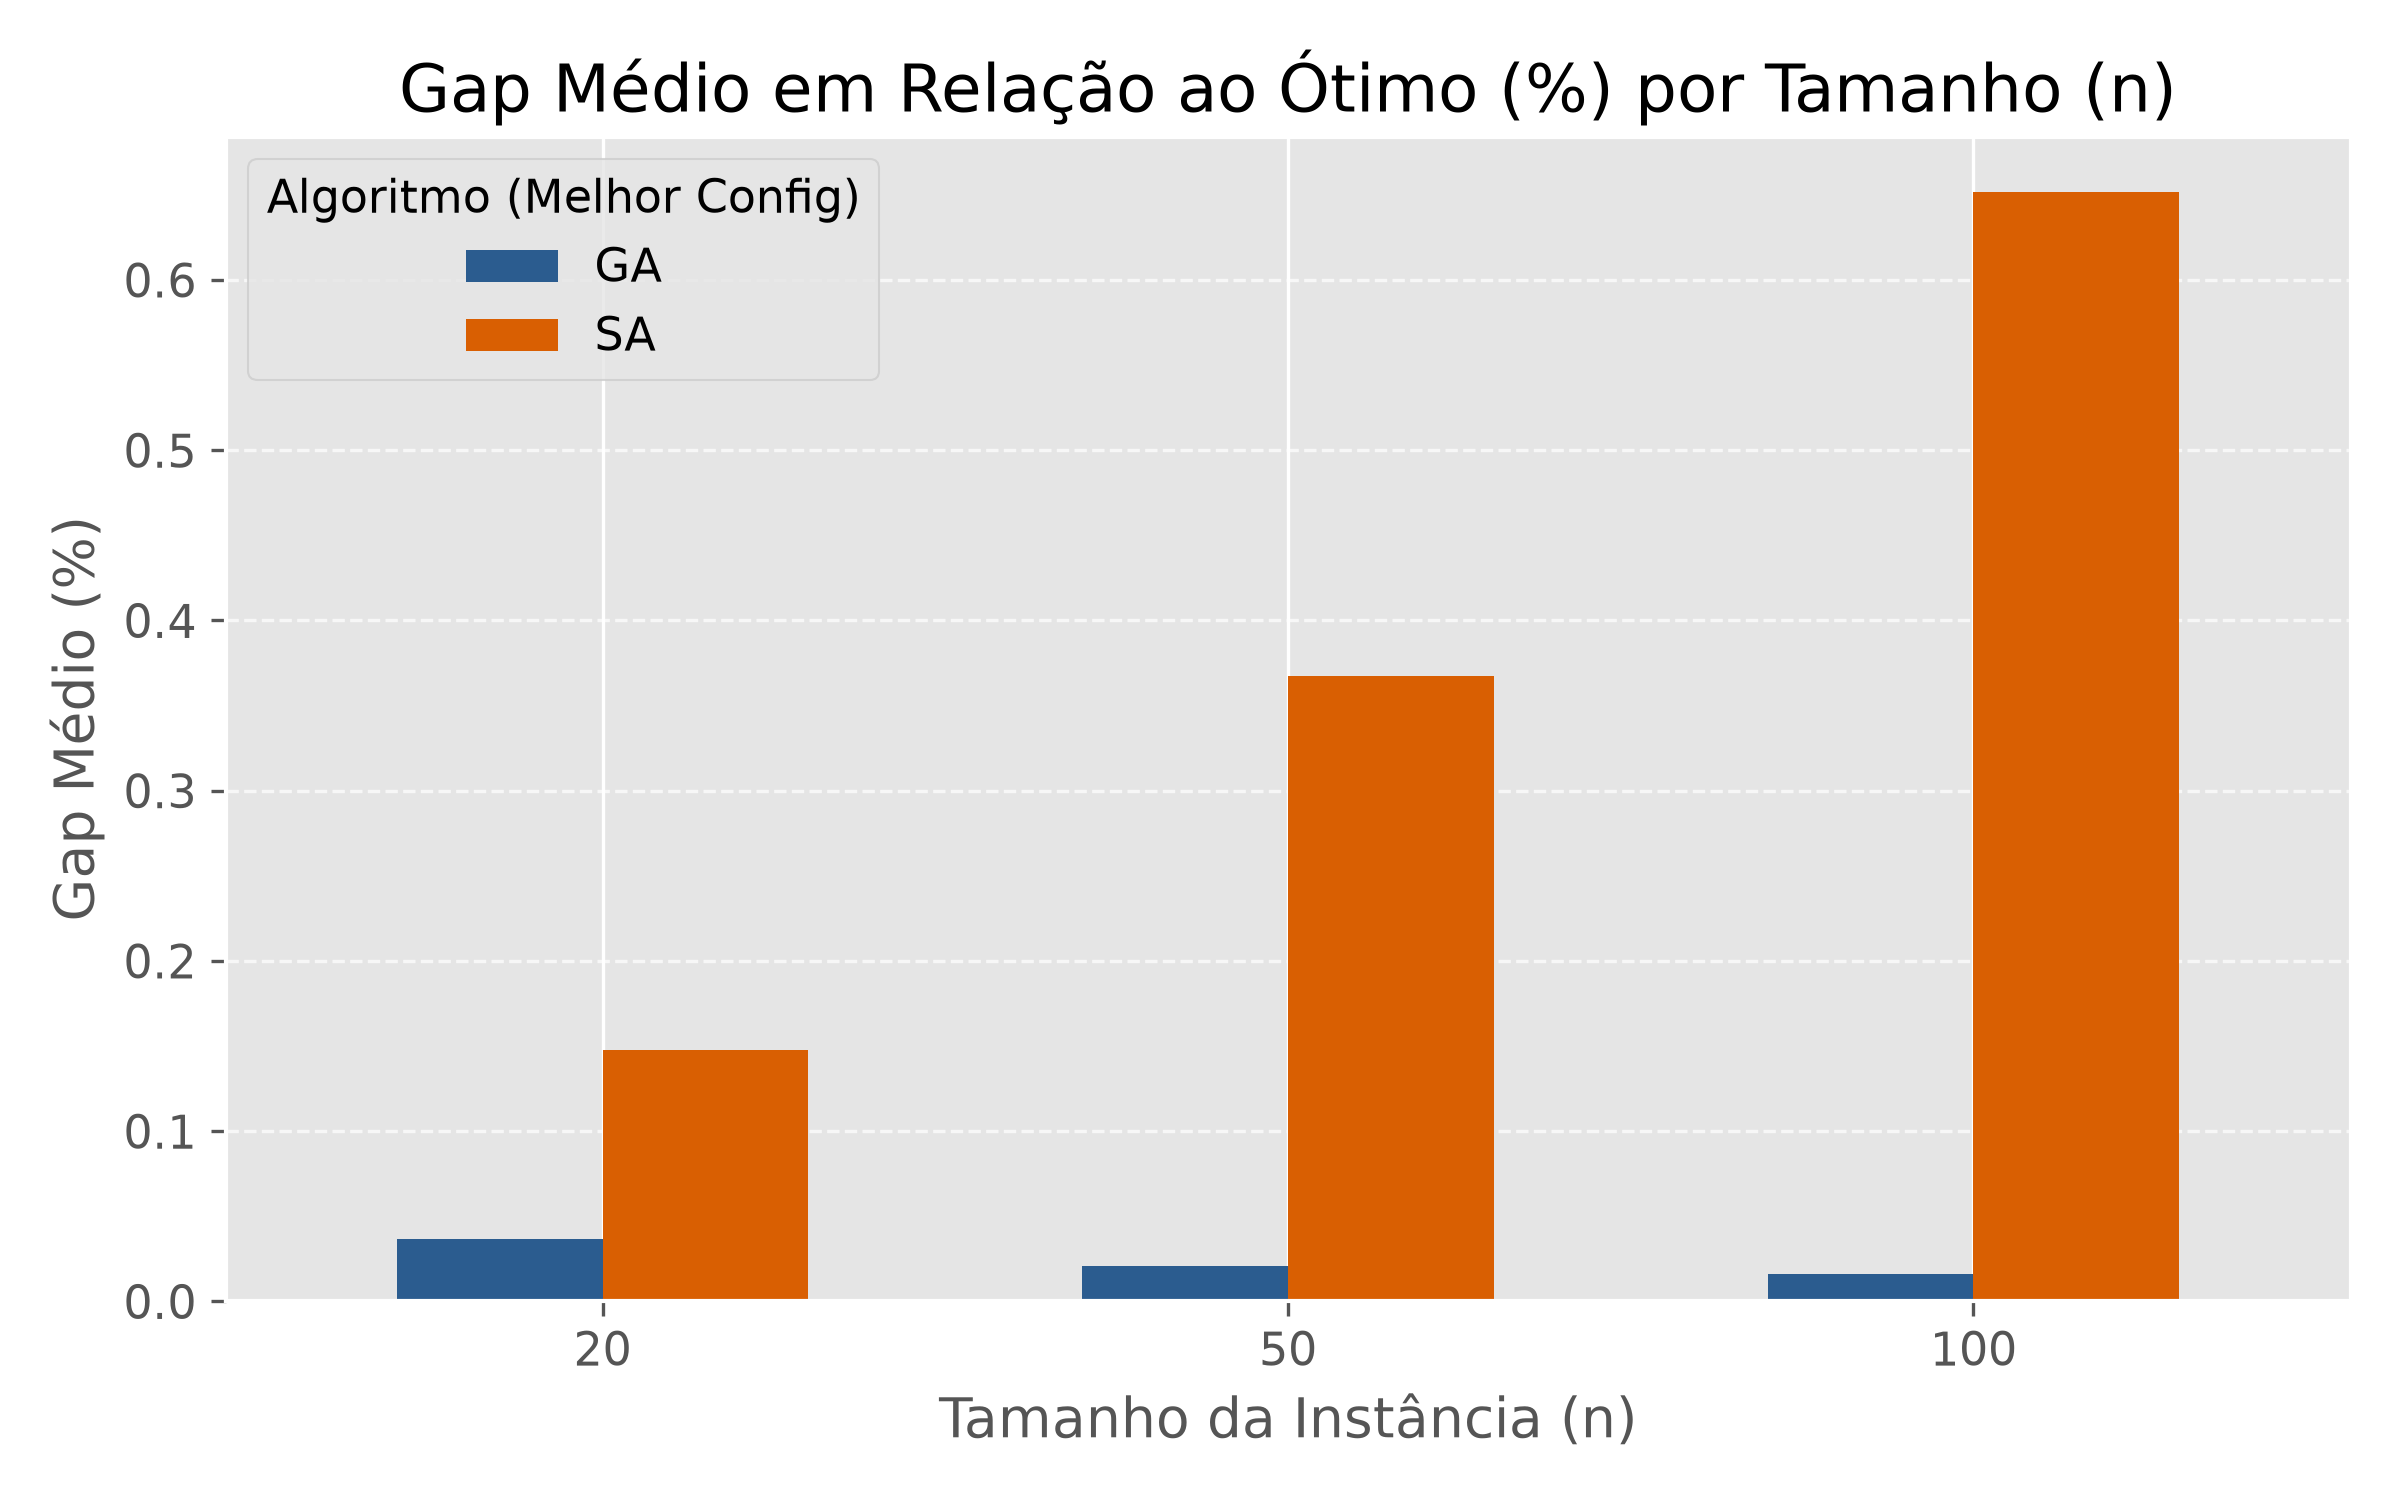
\includegraphics[width=0.80\textwidth]{../results/figures/gap_by_group.png}
\caption{Comparação do Gap Médio (\%) entre a melhor variante do GA e do SA por tamanho $n$.}
\label{fig:gap_final}
\end{figure}

\begin{figure}[H]
\centering
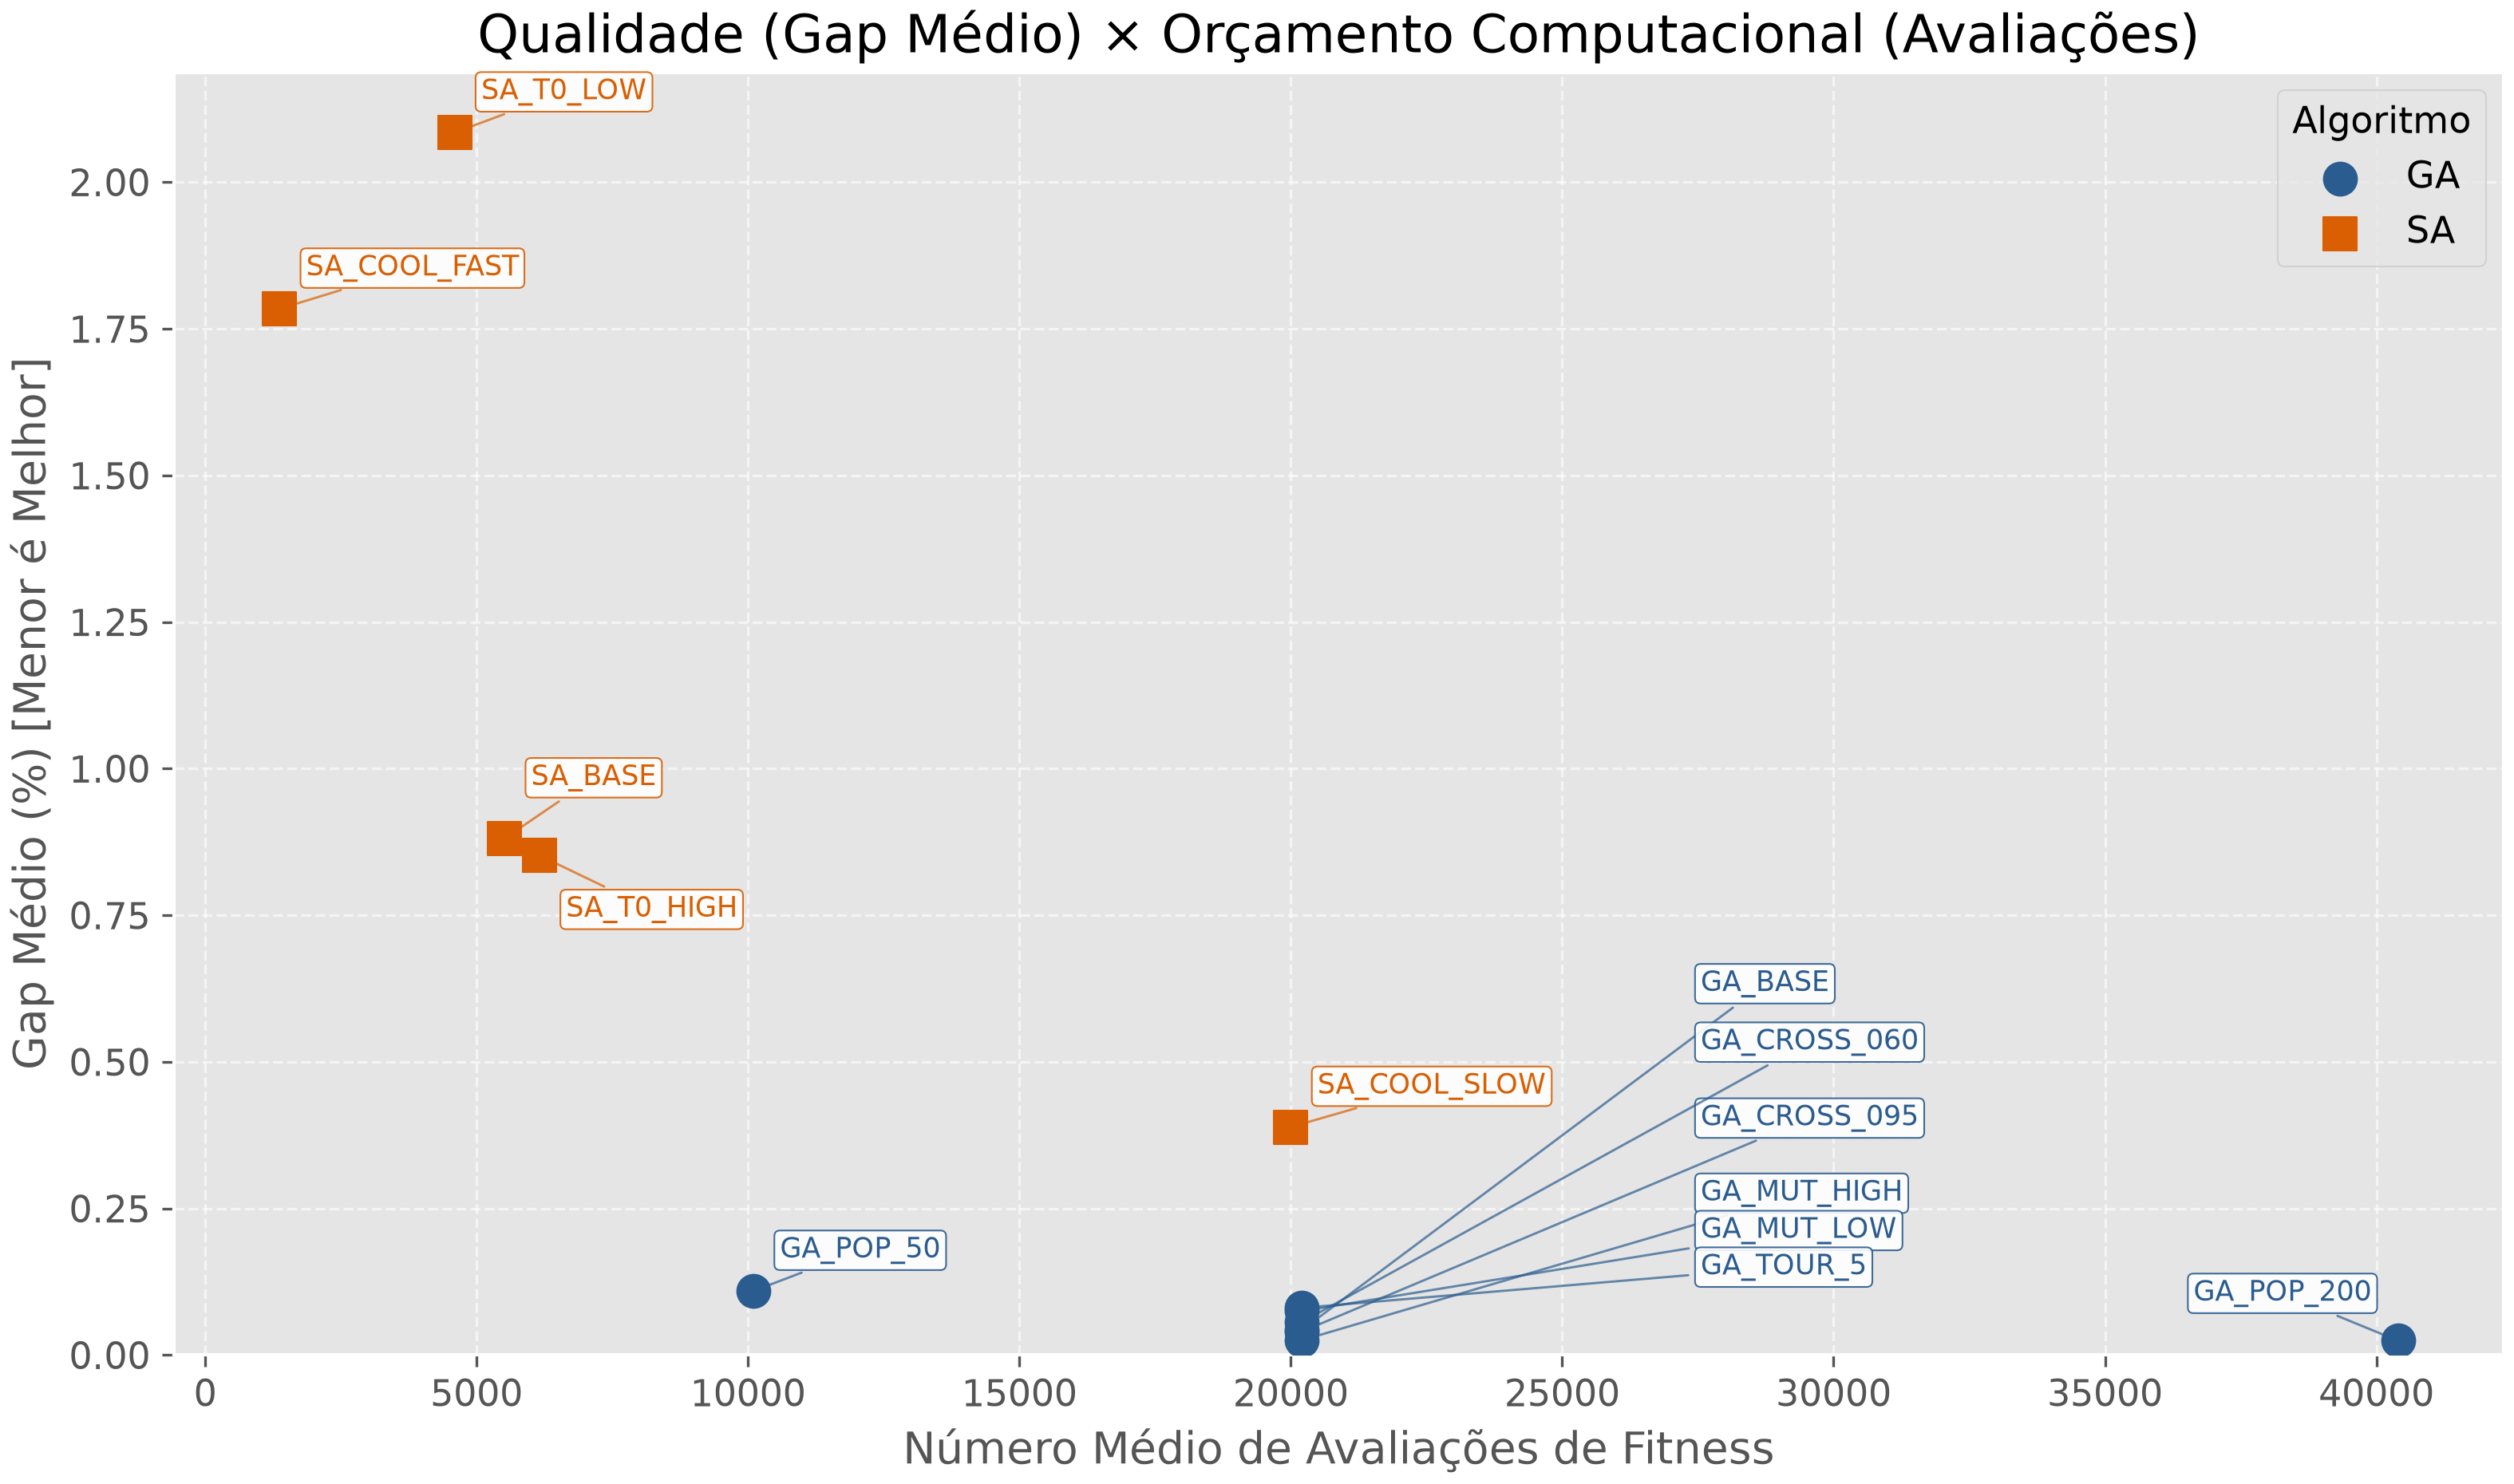
\includegraphics[width=0.90\textwidth]{../results/figures/pareto_quality_cost.png}
\caption{Qualidade (gap médio) em função do orçamento computacional, medido pelo número de avaliações.}
\label{fig:pareto}
\end{figure}

\paragraph{Discussão dos Trade-offs e Orçamento Computacional:}
\begin{enumerate}
    \item \textbf{Qualidade das Soluções e Escala ($n=20 \to 100$):} O GA apresentou gaps médios inferiores ao SA em todas as dimensões. Contudo, observa-se que o \texttt{GA\_POP\_200} consumiu 40.400 avaliações de fitness por execução, enquanto o \texttt{SA\_COOL\_SLOW} executou 20.002 avaliações.
    \item \textbf{Análise de Orçamento Controlado:} Ao comparar configurações sob orçamentos computacionais equivalentes na Figura~\ref{fig:pareto} (20.200 avaliações), a variante \texttt{GA\_MUT\_HIGH} ($P_m=2/n$) registrou gap médio de 0,0252\%, valor inferior ao obtido pelo \texttt{SA\_COOL\_SLOW} (0,3889\%). Esses dados são compatíveis com a hipótese de que a superioridade observada do paradigma GA no contexto deste experimento associa-se à recombinação por crossover, e não apenas ao aumento de avaliações.
    \item \textbf{Custo Computacional e Tempo:} O SA manteve tempos de execução inferiores aos do GA de 200 indivíduos (100,27 ms vs 321,92 ms em $n=100$), padrão condizente com a menor complexidade computacional da sua estrutura de vizinhança sem manipulação de populações.
\end{enumerate}

\section{Conclusão}

Este trabalho apresentou um estudo experimental abrangente sobre a resolução do Problema da Mochila 0/1 via Algoritmo Genético e Simulated Annealing. Por meio de um projeto experimental estruturado em 3 partes fundamentais envolvendo 90 instâncias verificadas com Programação Dinâmica e 11.700 execuções, foi possível compreender detalhadamente o efeito dos hiperparâmetros e os mecanismos de busca de cada algoritmo.

Os experimentos demonstraram que o aumento da população no GA ($N=200$) e a redução da taxa de resfriamento no SA ($\alpha=0.999$) foram decisivos para mitigar a convergência prematura. Na comparação final, o Algoritmo Genético (\texttt{GA\_POP\_200}) sobressaiu-se amplamente em qualidade de solução (gap médio global de 0,0245\% contra 0,3889\% do SA), enquanto o Simulated Annealing (\texttt{SA\_COOL\_SLOW}) destacou-se pela rapidez de execução.

Como trabalhos futuros, sugere-se a investigação de metaheurísticas híbridas (algoritmos meméticos), combinando a exploração populacional do GA com a busca local acelerada do SA.

\bibliographystyle{sbc}
\bibliography{referencias}

\end{document}
